\graphicspath{{chapters/12/images/}}
\chapter{The isobaric ensembles}

\section{Introduction}
The isobaric ensemble is useful in molecular dynamics as the subject of investigation are biological systems, therefore all simulation should run at constant temperature and pressure.

	\subsection{Legendre transform of E}
	In order to get to constant temperature and pressure the first step is to perform a Legendre transform of the energy, obtaining in this way the isobaric-isoentalpic ensemble.
	The same reasoning was made when the canonical ensemble was introduced from microcanonical one.

	$$\tilde{f}(s) = f(x(s))-sx(s)\qquad s = f'(x)$$

	The Legendre transform will be taken of the energy, with respect to to its derivative with respect to to its entropy.

	$$\tilde{E}(N, \frac{\partial E}{\partial V}, S) = E(N, V(P), S) - \biggl(\frac{\partial E}{\partial V}\biggr)_{N, S}V(N, \frac{\partial E}{\partial V}, S)$$

	So the Legendre transform should be expressed in term of the temperature: the derivative of the function with respect to its entropy.
	Pressure is being introduced as the derivative of the energy with respect to the volume.
	This function would contain the number of molecules and volume will be expressed in term of the pressure.
	Moreover defining the enthalpy as:

	$$H(N, P, S) = E(N, P, S) + PV(N, P, S)$$

	As it is usually done for thermodynamic potentials, its differential form is equal to:

	$$dH = dE + PdV + VdP = TdS - PdV + \mu dN + PdV + VdP$$

	From the first principle of thermodynamics:

	$$dE = TdS-PdV + \mu dN$$

	Where $\mu$ is the chemical potential.
	Then:

	$$dH = TdS + \mu dN + VdP$$

	From this the following derivatives can be obtained:

	$$T = \biggl(\frac{\partial H}{\partial S}\biggr)_{N, P} \qquad \langle V\rangle = \biggl(\frac{\partial H}{\partial P}\biggr)_{N, S} \qquad \mu = \biggl(\frac{\partial H}{\partial N}\biggr)_{P, S}$$

	The volume is averaged because in this ensemble it is not fixed, but will vary.

	\subsection{Legendre transform of A}
	 In the exact same way the Legendre transform can be applied to the Helmholtz free energy, with the formulas being very similar to before:

	$$\tilde{f}(s) = f(x(s))-sx(s)\qquad s = f'(x)$$

	Again it is a Legendre transform with respect to its derivative with respect to volume, so the derivative of $A$ with respect to to volume.
	This derivative is related to the pressure, so the Legendre transform will be equal to the Helmholtz itself, minus the derivative of $A$ with respect to volume times volume, which will be expressed in terms of the derivative of $A$ with respect to to volume:

	$$\tilde{A}(N, \frac{\partial A}{\partial V}, T) = A(N, V(P), T)- \biggl(\frac{\partial A}{\partial V}\biggr)_{N, T}V(N, \frac{\partial A}{\partial V}, T)$$

	A thermodynamic potential is derived, that is called Gibbs free energy:

	$$G(N, P, T) = A(N, P, T) + PV(N, P, T)$$

	The Gibbs free energy is the Legendre transform of the $A$, like the enthalpy is the Legendre transform of the energy.
	Considering now the infinitesimal variation of $G$:

	$$dG = dA + PdV + VdP = -PdV + \mu dN - SdT + PdV + VdP$$

	Like before, the $PdV$ cancel out:

	$$dG = \mu dN + VdP - SdT$$

	Considering now the thermodynamics derivatives:

	$$S = -\biggl(\frac{\partial G}{\partial T}\biggr)_{N, P}\qquad\langle V\rangle = \biggl(\frac{\partial G}{\partial P}\biggr)_{N, T}\qquad \mu = \biggl(\frac{\partial G}{\partial N}\biggr)_{P, T}$$

	Obtaining as a result:

	\begin{itemize}
	\item The isobaric-isoenthalpic ensemble as a Legendre transform of the microcanonical ensemble;
	\item The isobaric-isothermal ensemble as the Legendre transform of the canonical ensemble.
	\end{itemize}

	This is the same process to follow when changing simulation: it has to be noted that molecular simulations are carried in the NPT ensemble.

	\subsection{Phase space distribution of the isoenthalpic-isobaric ensemble}
	Pressure and enthalpy are kept fixed as the energy and the volume where in the microcanonical ensemble.
	The conserved quantity is therefore $H$, the enthalpy:

	$$H = \mathcal{H}(v) + PV$$

	The phase-space distribution must be the solution for the Liouville equation.
	This is some function of the Hamiltonian.
	Because $H$ will be kept fixed and it is itself a function of the Hamiltoninan, the solutio will be:

	$$f(x) = F(\mathcal{H}(x)) = \mathcal{M}\delta(\mathcal{H}(x)+PV-H)$$

	Now considering a function analogous to the configuration of the microcanonical ensemble, similar to the $\Omega$.
	The pressure varies from $0$ to $\infty$, so there is a need to integrate the constant enthalpy hypersurface over the volume:

	$$\Gamma(N, P, H) = \mathcal{M}\int_0^{\infty}dV\int d^N\vec{p}\int_{\mathcal{D}(V)}d^N\vec{r}\delta(\mathcal{H}(\vec{r}, \vec{p}) + PV-H)$$

	The integral $\int_0^{\infty}dV$ is on the left side of the equation because the molecules (coordinates) are integrated over the volume, depending on it.
	This is very similar to the microcanonical ensemble, when the function $\Omega$ was correlated to the entropy.
	This process can be repeated obtaining the Boltzmann relation.
	The entropy as a function of the number of particles, the pressure and the enthalpy are:

	$$S(N, P, H) = k \ln \Gamma(N, P, H)$$

	$$dH = TdS + \mu dN + VdP$$

	All the thermodynamics derivatives can be derived and the system described:

	$$\frac{1}{T} = \biggl(\frac{\partial S}{\partial H}\biggr)_{N, P}\qquad \frac{\langle V\rangle}{T} = -\biggl(\frac{\partial S}{\partial P}\biggr)_{N, H}\qquad \frac{\mu}{T} = -\biggl(\frac{\partial S}{\partial N}\biggr)_{P, H}$$

\section{Isothermal-isobaric ensemble}
Considering now the isothermal-isobaric ensemble the thermodynamics variables have to be written down.
The reasoning behind this derivations is the same of the canonical and microcanonical ensemble.
Now the objective is to go from the analogous microcanonical (isobaric-isoenthalpic) to the analogous canonical (isothermal-isobaric).
Figure \ref{fig:isobar} proves the similarity between the system, with the only difference being the piston at the bottom, since the pressure is not constant in both compartment.

\begin{figure}
\center
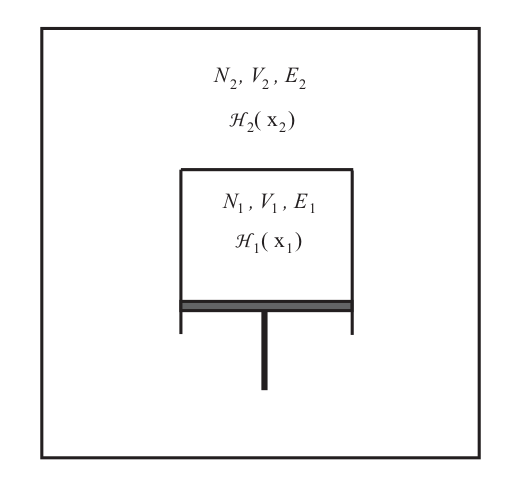
\includegraphics[scale=0.4]{isobar}
\label{fig:isobar}
\caption{Two systems in contact with a common thermal reservoir at temperature T. System
$1$ has $N_1$ particles in a volume $V_1$ ; system $2$ has $N_2$ particles in a volume $V_2$. Both $V_1$ and $V_2$ can vary.}
\end{figure}

\begin{multicols}{2}
	\begin{itemize}
		\item $E = E_1 + E_2\quad E_2\gg E_1$.
		\item $N = N_1 + N_2\quad N_2\gg N_1$.
		\item $V = V_1 + V_2\quad V_2\gg V_1$
		\item $\mathcal{H}(x) = \mathcal{H}_1(x_1) + \mathcal{H}_2(x_2)$.
	\end{itemize}
\end{multicols}


At fixed volumes $V_1$ and $V_2$:

$$Q(N, V, T) = C_N\int dx_1dx_2 e^{-\beta[\mathcal{H}_1(x_1) + \mathcal{H}_2(x_2)]} = g(N, N_1, N_2)C_{N_1}\int dx_1 e^{-\beta\mathcal{H}_1(x_1)}C_{N_2}\int dx_2 e^{-\beta\mathcal{H}_2(x_2)}$$

Which is the same expression for the microcanonical ensemble.
$C_{N_1}$ and $C_{N_2}$ are the two constants that are needed to separate the system in two canonical ensemble with the same temperature $\beta$.
The partition function for the system is:

$$Q(N, V, T) \propto Q(N_1, V_1, T)Q(N_2, V_2, T)$$

	\subsection{Phase space distribution}
	Now allowing the volume to change and considering the combined system:

	$$f(x) = \frac{C_Ne^{-\beta\mathcal{H}(x)}}{Q(N, V, T)} = \frac{g(N, N_1, N_2)}{Q(N, V, T)}C_{N_1}e^{-\beta\mathcal{H}_1(x_1)}C_{N_2}e^{-\beta\mathcal{H}_2(x_2)}$$

	To simplify the variables that describe the system $2$ there is a need to integrate over the $x_2$ variables.

	$$f(x_1) = \frac{g(N, N_1, N_2)}{Q(N, V, T)}C_{N_1}e^{-\beta\mathcal{H}_1(x_1)}C_{N_2}\int dx_2 e^{-\beta\mathcal{H}_2(x_2)} = \frac{Q_2(N_2, V-V_1, T)}{Q(N, V, T)}g(N, N_1, N_2)C_{N_1}e^{-\beta\mathcal{H}_1(x_1)}$$

	The quantity $C_{N_2}\int dx_2 e^{-\beta\mathcal{H}_2(x_2)}$ is exactly the partition function for the system $2$, considered as a canonical ensemble, with a fixed number of particles and a given volume and temperature.
	Thus being equal to $Q_2$: considering now this quantity.
	First, the normalization is correct: $\int dV_1\int dx_1f(x_1, V_1) = 1$.
	Generally the partition function ($Q_2$ in this case) is equal to $e^{\beta[A]}$.
	Writing this equation with the correct argument for the Helmholtz free energy.

	$$\frac{Q_2(N_2, V-V_1, T)}{Q(N, V, T)} = e^{-\beta[A(N-N_1, V-V_1, T) - A(N, V, T)]}$$

	Through a Taylor expansion:

	$$A(N-N_1, V-V_1, T) = A(N, V, T)-N_1\frac{\partial A}{\partial N}|_{N_1 = 0, V_1 = 0} = A(N, V, T)-\mu N_1 + PV_1$$

	The phase-space distribution for variable $x_1$ is:

	$$f(x_1) = g(N, N_1, N-N_1) e^{\beta\mu N_1}e^{-\beta P V_1}C_{N_1}e^{-\beta\mathcal{H}_1(x_1)}\qquad I_{N_1} = \frac{1}{V_0N_1!h^{3N_1}}$$

	A quantity $\Delta(N, P, T)$ is defined to be the integral of the entire phase-space, including the volume, of the constant $I_N$.
	The phase-space distribution is $e^{-\beta(\mathcal{H}(x) + PV)}$: the analogous distribution function of the canonical ensemble, but instead of having the energy in the Boltzmann factor there is the enthalpy:

	$$\Delta(N, P, T) = I_N\int_0^{\infty}dV\int dxe^{-\beta(\mathcal{H}(x) + PV)}\Rightarrow e^{\beta\mu N}\Delta(N, P, T) = 1$$

	Because of Euler, the quantity $\mu N$ is exactly $G$:

	$$\Delta(N, P, T) = e^{-\beta\mu N} = e^{-\beta G(N, P, T)}$$

	Now an analogous relation has been obtained: $e^{\beta A} \rightarrow e^{\beta G}$.
	And:

	$$\Delta(N, P, T) = \frac{1}{V_0N!h^{3N}}\int_0^{\infty}dVe^{-\beta PV}\int dxe^{-\beta\mathcal{H}(x)} = \frac{1}{V_0}\int_0^{\infty}dVe^{-\beta PV}Q(N, V, T)$$

	\subsubsection{Further proof}
	A further proof that this is indeed a "good" system is provided, starting this time from the Gibbs free energy:

	$$G = A + P\langle V \rangle = \langle E + PV\rangle - TS = \langle\mathcal{H}(x) + PV\rangle + T\frac{\partial G}{\partial T}$$

	The average $langle E + PV\rangle$ can be obtained by performing the average over the phase-space distribution just introduced.
	There is a need to integrate over the volume and all the coordinates.
	The quantity $(\mathcal{H}(x) + PV)$ (remember that $V$ now is a constant) must be weighted by the corresponding Boltzmann factor, which includes not only the Hamiltonian but also $PV$.

	$$\langle E + PV\rangle = \frac{I_N\int_0^{\infty} dV\int dx(\mathcal{H}(x) + PV)e^{-\beta(\mathcal{H}(x)+PV)}}{I_N\int_0^{\infty}dV\int dxe^{-\beta(\mathcal{H}(x) + PV)}} = -\frac{1}{\Delta(N, P, T)}\frac{\partial \Delta(N, P, T)}{d\beta} = -\frac{\partial\ln\Delta(N, P, T)}{\partial \beta}$$


	$$G(N, P, \beta) = -\frac{\partial\ln\Delta(N, P, \beta)}{\partial\beta}-\beta\frac{\partial G}{\partial \beta}$$

	Plugging in the following solution: $G(N, P, \beta) = -\frac{1}{\beta}\ln\Delta(N, P, \beta)$ in the previous differential equation we get $0$.
	Now the system can be described:

	$$\langle V\rangle = \biggl(\frac{\partial G}{\partial P}\biggr)_{N, T}\qquad S = -\biggl(\frac{\partial G}{\partial T}\biggr)_{N, P}$$

	\subsection{Maxwell's square}
	Putting everything into perspective: in the NPT ensemble the average volume can be obtained as the derivative with respect to pressure of the Gibbs free energy and entropy can be taken as the derivative with respect to temperature keeping fixed $N$ and $T$:
	Let's put everything into perspective.

	\begin{multicols}{2}
		\begin{itemize}
			\item $\langle V\rangle = \biggl(\frac{\partial G}{\partial P}\biggr)_{N, T}$.
			\item $S = -\biggl(\frac{\partial G}{\partial T}\biggr)_{N, P}$.
		\end{itemize}
	\end{multicols}

	Moreover the following equations from the isobaric-isoenthalpic ensemble where found:

	\begin{multicols}{2}
		\begin{itemize}
			\item $T = \biggl(\frac{\partial H}{\partial S}\biggr)_{N, P}$.
			\item $\langle V\rangle = \biggl(\frac{\partial H}{\partial P}\biggr)_{N, S}$.
		\end{itemize}
	\end{multicols}

	While the following are coming from the microcanonical ensemble:

	\begin{multicols}{2}
		\begin{itemize}
			\item $T = =\biggl(\frac{\partial U}{\partial S}\biggr)_{N, V}$.
			\item $P = - \biggl(\frac{\partial U}{\partial V}\biggr)_{N, S}$.
		\end{itemize}
	\end{multicols}

	And the canonical ensemble:

	\begin{multicols}{2}
		\begin{itemize}
			\item $P = -\biggl(\frac{\partial A}{\partial V}\biggr)_{N, T}$.
			\item $S = - \biggl(\frac{\partial A}{\partial T}\biggr)_{N, V}$.
		\end{itemize}
	\end{multicols}

	\begin{figure}[H]
		
\includegraphics[scale = 0.1]{maxwell_square}
		\centering
		\caption{Maxwell's square}
	\end{figure}


	\subsection{Pressure viral theorem}
	The internal pressure that was calculated by the estimator was a function of all the coordinates and all the momenta.
	The internal pressure $P^{int}$ would be the average of this estimator.
	This quantity should be equal to the external pressure for the equations to be valid:

	$$P^{(int)} =\langle\mathcal{P}(\vec{r}, \vec{p})\rangle = \biggl\langle\frac{1}{3V}\sum\limits_i\biggl[\frac{\vec{p}_i^2}{m_i} + \vec{F}_i\cdot\vec{r}_i\biggr]\biggr\rangle = kT\frac{\partial\ln Q}{\partial V}$$

	To take average of this quantity for our new ensemble (NPT) the partition function should be put at the denominator and then there should be an integration over the volume.

	\begin{align*}
		\langle P^{(int)}\rangle &= \frac{1}{\Delta(N, P, T)}\int_0^{\infty}dVe^{-\beta PV}Q(N, V, T)\frac{kT}{Q}\frac{\partial Q}{\partial V} = \frac{kT}{\Delta(N, P, T)}\int_0^{\infty}dVe^{-\beta PV}\frac{\partial Q}{\partial V}=\\
														 &= \frac{kT}{\Delta(N, P, T)}e^{-\beta PV}Q(N, V, T)|_0^{\infty}-\frac{kT}{\Delta(N, P, T})\int_0^{\infty}dV\biggl(-\frac{P}{kT}\biggr)e^{-\beta PV}Q(N, V, T) = \\
														 &=\frac{P}{\Delta(N, P, T)}\int_0^{\infty}dVe^{-\beta PV}Q(N, V, T) = P
	\end{align*}

	Consider the integration by parts of the quantity $\frac{kT}{\Delta(N, P, T)}e^{-\beta PV}Q(N, V, T)|_0^{\infty}$: when the volume tends to $\infty$ the exponential goes to zero; when instead the volume is zero the partition function is zero, because there are no states where $V=0$.
	Now only the second term is there and its integral is exactly $\Delta$.
	Again, the quantity $dVe^{-\beta PV}Q(N, V, T)$ is equal to $\Delta$, obtaining the external pressure $P$.
	Considering that taking the average of the internal pressure over the NPT ensemble exactly the external pressure $P$ is obtained, this is the expected result.
	 This also means that when comparing the result of the simulation with the external pressure that is being fixed, the internal pressure should be computed and then its average over many simulations.
	 So, in conclusion, the volume-average internal pressure is equal o the external one.

	\subsection{Work Virial theorem}
	Multiplying the internal pressure for the changing volume:

	$$P^{(int)}V = kTV\frac{\partial \ln Q}{\partial V}$$

	The same equation as before are obtained, but with the inclusion of $V$:

	\begin{align*}
		\langle P^{(int)}V\rangle &= \frac{1}{\Delta(N, P, T)}\int_0^{\infty}dVe^{-\beta PV}Q(N, V, T)\frac{kTV}{Q}\frac{\partial Q}{\partial V} = \frac{kT}{\Delta(N, P, T)}\int_0^{\infty}dVe^{-\beta PV}V\frac{\partial Q}{\partial V} = \\
															&=\frac{kT}{\Delta(N, P, T)}e^{-\beta PV}VQ(N, V, T)|_{0}^{\infty}-\frac{kT}{\Delta(N, P, T)}\int_0^{\infty}dV\frac{\partial}{\partial V}(Ve^{-\beta PV})Q(N, V, T)=\\
															&= \frac{1}{\Delta(N, P, T)}\biggl[-kT\int_0^{\infty}dVe^{-\beta PV}Q(N, V, T) + P\int_0^{\infty}dV \, Ve^{-\beta PV}Q(N, V, T)\biggr]=\\
															&=-kT+P\langle V\rangle \Rightarrow \langle P^{(int)}V\rangle + kT = P\langle V\rangle
	\end{align*}

	The term $\int_0^{\infty}dV \, Ve^{-\beta PV}Q(N, V, T)$ is the average of the volume: the volume is multiplied by a weighting factor and divided by the partition function in the NPT ensemble.
	The work is equal to the average quantity $\langle P^{(int)}V\rangle$, plus $kT$.
	Now, $kT$ indicates that is equation is the analogous of the equipartition theorem, but there's an extra degree of freedom, the varying volume.
	This is the reason why an additional $kT$ is present.
	To be fair, $kT$ is very small and it does not change much the final equation.
	In conclusion it can be seen how there is an extra degree of freedom, the volume.
	These theorems are particularly important, since the algorithms described later are all written for the isobaric-isoenthlapic ensemble, but are easily obtained adding a thermostat.

\section{Andersen's Hamiltonian}
The best way to deal with the volume as an extra degree of freedom is to add it to the Hamiltonian as an extra variable, obviously with its own momentum.
This is the case of the Andersen's Hamiltonian, defined as:

$$\mathcal{H}_A = \sum\limits_{i=1}^N\frac{V^{-\frac{2}{3}}\pi_i^2}{2m_i}+ U(V^\frac{1}{3}\vec{s}_1, \dots, V^{\frac{1}{3}}\vec{s}_N) + \frac{p_V^2}{2W} + PV\qquad W = (3N+1)kT\tau_b^2$$

Hamilton's equation has to be written down to obtain the time evolution for each of these coordinates:

\begin{itemize}
	\item $\dot{\vec{s}}_i = \frac{\partial \mathcal{H}_A}{\partial\pi_i} = \frac{V^{-\frac{2}{3}}\pi_i}{m_i}$.
	\item $\dot{\pi}_i = -\frac{\partial\mathcal{H}_A}{\partial\vec{s}_i} = -\frac{\partial U}{\partial (V^{\frac{1}{3}}\vec{s}_i)}V^{\frac{1}{3}}$.
	\item $\dot{V} = \frac{\partial\mathcal{H}_A}{\partial p_V}-\frac{p_V}{W}$.
	\item $\dot{p}_V = -\frac{\partial\mathcal{H}_A}{\partial V} = \frac{1}{3}V^{-\frac{5}{3}}\sum\limits_{i=1}^N\frac{\pi_i^2}{m_i}-\frac{1}{3}V^{-\frac{2}{3}}\sum\limits_{i=1}^N\frac{\partial U}{\partial(V^{\frac{1}{3}}\vec{s}_i)}\cdot\vec{s}_i-P$.
\end{itemize}

The derivative of $\dot{p}_V$ is slightly more complicated, since the dependence on $p$ is present on three terms.
Inverting the transformation (the same inversion we performed to go from original coordinates to the scaled coordinates):

$$s_i = V^{-\frac{1}{3}}\vec{r}_i\Rightarrow \dot{\vec{s}}_i = V^{-\frac{1}{3}}\dot{\vec{r}}_i-\frac{1}{3}V^{-\frac{4}{3}}\dot{V}\vec{r}_i$$

$$\pi_i = V^{\frac{1}{3}}\vec{p}_i \Rightarrow \dot{\pi}_i = V^{\frac{1}{3}}\dot{\vec{p}}_i + \frac{1}{3}V^{-\frac{2}{3}}\dot{V}\vec{p}_i$$

Now these equations need to be substituted to the ones that were previously derived:

\begin{itemize}
	\item $\dot{\vec{s}}_i = \frac{\partial \mathcal{H}_A}{\partial\pi_i} = \frac{V^{-\frac{2}{3}}\pi_i}{m_i} \rightarrow \dot{r}_i = \frac{p_i}{m_i} + \frac{\dot{V}}{3V} r_i$
	\item $\dot{\pi}_i = -\frac{\partial\mathcal{H}_A}{\partial\vec{s}_i} = -\frac{\partial U}{\partial (V^{\frac{1}{3}}\vec{s}_i)}V^{\frac{1}{3}} \rightarrow \dot{p}_i = - \frac{\partial U}{\partial r_i} - \frac{\dot{V} }{3V} p_i$ .
	\item $\dot{V} = \frac{\partial\mathcal{H}_A}{\partial p_V}-\frac{p_V}{W} \rightarrow \dot{V} = \frac{p_V}{W}$.
	\item $\dot{p}_V = -\frac{\partial\mathcal{H}_A}{\partial V} = \frac{1}{3}V^{-\frac{5}{3}}\sum\limits_{i=1}^N\frac{\pi_i^2}{m_i}-\frac{1}{3}V^{-\frac{2}{3}}\sum\limits_{i=1}^N\frac{\partial U}{\partial(V^{\frac{1}{3}}\vec{s}_i)}\cdot\vec{s}_i-P \rightarrow \dot{p}_V = \frac{1}{3V} \sum^N_{i=1} [\frac{p^2_i}{m_i} - \frac{\partial U}{\partial r_i} r_i] -P$.
\end{itemize}

Notice how the new term $ \frac{\dot{V}}{3V}$ accounts for the compressibility of the variable, letting it inflate and deflate.
Notice that the last quantity is exactly the internal pressure estimator.
Now a variation in the momentum is present, that is conjugate to the volume, whenever the internal pressure differs from the external one ($\dot{p} != 0$).
The compressibility is equal to $0$ so the system is incompressible.
To calculate the compressibility the derivative of $\dot{r}$ with respect to $r_i$ has to be computed.
This yields the factor $\frac{\dot{V}}{3V}$ for each particle and every degree of freedom, which are three for each particle.

	\subsection{Andersen's equations}

	\begin{multicols}{2}
		\begin{itemize}
			\item $\dot{\vec{r}}_i = \frac{\vec{p}}{m_i} + \frac{\dot{V}}{3V}\vec{r}_i\Rightarrow\dot{\vec{r}}_i = \frac{\vec{p}_i}{m_i} + \frac{\dot{V}}{3V}\vec{r}_i$
			\item $\dot{\vec{p}}_i = -\frac{\partial U}{\partial\vec{r}_i} -\frac{\dot{V}}{3V}\vec{p}_i\Rightarrow \dot{\vec{p}}_i = -\frac{\partial U}{\partial\vec{r}_i}-\frac{\dot{V}}{3V}\vec{p}_i$.
			\item $\dot{V} = \frac{p_V}{W}\Rightarrow\dot{V} = \frac{p_V}{W}$.
			\item $\dot{p}_V = \frac{1}{3V}\sum\limits_{i=1}^N\biggl[\frac{\vec{p}_i^2}{m_i}-\frac{\partial U}{\partial\vec{r}_i}\cdot\vec{r}_i\biggr]-P\Rightarrow\dot{p}_V = \frac{1}{3V}\sum\limits_{i=1}^N\biggl[\frac{\vec{p}_i^2}{m_i}-\frac{\partial U}{\partial\vec{r}_i}\cdot\vec{r}_i\biggr]-P$.
		\end{itemize}
	\end{multicols}

	The conserved quantity:

	$$\mathcal{H}' = \sum\limits_{i=1}^N\frac{\vec{p}_i^2}{2m_i} + U(\vec{r}_1, \dots, \vec{r}_N) + \frac{p_V^2}{2W}+PV$$

	Notice how $\mathcal{H}'$ looks very similar to the enthalpy, aside from the kinetic energy part.
	As usual, when working in a system that is not Hamiltonian, since if it was obtained from a different Hamiltonian, $\mathcal{H}'$ does not give back Anderson's equations, the partition function has to be derived:

	$$\Omega_P = \int dp_V\int_0^{\infty}\int d^N\vec{p}\int_{\mathcal{D}(V)}d^N\vec{r}\delta\biggl(\\mathcal{H}(\vec{r},\vec{p}) + \frac{p_V^2}{2W}+PV-H\biggr)$$

	According to the Virial theorem:

	$$\biggl\langle\frac{p_V^2}{2W}\biggr\rangle = k\frac{T}{2}\Rightarrow \mathcal{H}(\vec{r},\vec{p}) + PV\text{ is conserved}$$

	The average of the pressure will be kept constant, as for the enthalpy.

\section{MTK algorithm (NPT)}
One of the best choices for thermostatting the system is the MTK algorithm, developed by Martyna-Tobias-Klein in 1994.
This algorithm introduces a new variable $\epsilon$:

$$\epsilon = \frac{1}{3}\ln\frac{V}{V_0}\Rightarrow\dot{\epsilon} = \frac{\dot{V}}{3V}=\frac{p_\epsilon}{W}$$

\begin{multicols}{2}
	\begin{itemize}
		\item $\dot{\vec{r}}_i = \frac{\vec{p}_i}{m_i} + \frac{p_\epsilon}{W}\vec{r}_i$.
		\item $\dot{\vec{p}}_i = -\frac{\partial U}{\partial\vec{r}_i} - \frac{p_\epsilon}{W}\vec{p}_i$.
		\item $\dot{V} = \frac{dVp_\epsilon}{W}$.
		\item $\dot{p}_\epsilon = dV(\mathcal{P}^{(int)}-P)$.
	\end{itemize}
\end{multicols}


Considering compressibility:

\begin{align*}
	\kappa & = \sum\limits_{i=1}^N\biggl[\frac{\partial}{\partial\vec{r}_i}\cdot\dot{\vec{r}}_i + \frac{\partial}{\partial\vec{p}_i}\cdot\dot{\vec{p}}_i\biggr] + \frac{\partial\dot{V}}{\partial V} + \frac{\partial\dot{p}_V}{\partial p_V} = \\
				 &= dN\frac{p_\epsilon}{W}-dN\frac{p_\epsilon}{W} = d\frac{p_\epsilon}{E} = \frac{\dot{V}}{V}
\end{align*}

To obtain the incompressible equations that conserve $\mathcal{H}(\vec{r},\vec{p}) + PV + \frac{p_V^2}{2W}$ some modifications have to be applied:

$$\dot{\vec{p}}_i = -\frac{\partial U}{\partial\vec{r}_i} - \biggl(1+\frac{d}{N_F}\biggr)\frac{p_\epsilon}{W}\vec{p}_i\qquad \dot{p}_\epsilon = dV(\mathcal{P}^{(int)}-P) + \frac{d}{N_f}\sum\limits_{i=1}^N\frac{\vec{p}_i^2}{m_i}$$

With $F$ being the number of degrees of freedom of the system.

	\subsection{Langevin piston}
	In many programs and applications  the Langevin thermostat will be used.
	The only equation different from Andersen's ones is the last, with a friction acting on the volume and a last term representing a random force or ``kick".

	\begin{itemize}
		\item $\dot{\vec{r}}_i = \frac{\vec{p}_i}{m_i} + \frac{\dot{V}}{3V}\vec{r}_i$.
		\item $\dot{\vec{p}}_i = -\frac{\partial U}{\partial\vec{r}_i}-\frac{\dot{V}}{3V}\vec{p}_i$.
		\item $\dot{V} = \frac{p_V}{W}$.
		\item $\dot{p}_V = \frac{1}{3V}\sum\limits_{i=1}^N\biggl[\frac{\vec{p}_i^2}{m_i}-\frac{\partial U}{\partial\vec{r}_i}\cdot\vec{r}_i\biggr]-P-\gamma\dot{V}+R(t)$.
	\end{itemize}

	$$\langle R(0)R(t)\rangle = \frac{2\gamma kT}{W}\delta(t)$$

	The Langevin piston is mostly preferred as a barostat.

\section{Summary}

\begin{multicols}{2}
	\begin{itemize}
		\item The formalism of the isobaric ensembles has been constructed, starting by performing the Legendre transform of the microcanonical ensemble to obtain the isobaric-isoenthalpic enable; then the same reasoning was applied to the canonical ensemble to obtain the isobaric-isothermal (NPT) ensemble.
		\item It was demonstrated that the steps and the reasoning to modify the equations of the microcanonical ensemble to go to the canonical ensemble, apply in the same way also for the isobaric-isoenthalpic in the NPT.
		\item In the NPT ensemble everything can be computed like a canonical ensemble, however the volume is now a variable.
		\item The pressure Virial theorem, important for molecular simulations, and work Virial theorem, useful for the derivation of Andersen's Hamiltonian, were introduced.
		\end{itemize}
\end{multicols}
